\subsection{Temperature Abhängigkeit von $I_\mathrm{c}$ und $T_\mathrm{c}$}
Um die Temperaturabhängikeit der Größen $I_\mathrm{c}$ und $T_\mathrm{c}$ zu bestimmen werden bei verschiedenen Temperaturen die Strom-Spannungs-Kennlinien aufgenommen. An dieser Kennlinie sind insgesamt drei Sprünge zu sehen. Einer befindet sich am Ursprung und hat eine Höhe von $2 I_\mathrm{c}$. Die anderen beiden Sprünge befinden sich bei $V = \pm 2\Delta/e$. Dies ist in Abbildung \ref{fig:IVT} zu sehen.
\begin{figure}[H]
    \begin{centering}
        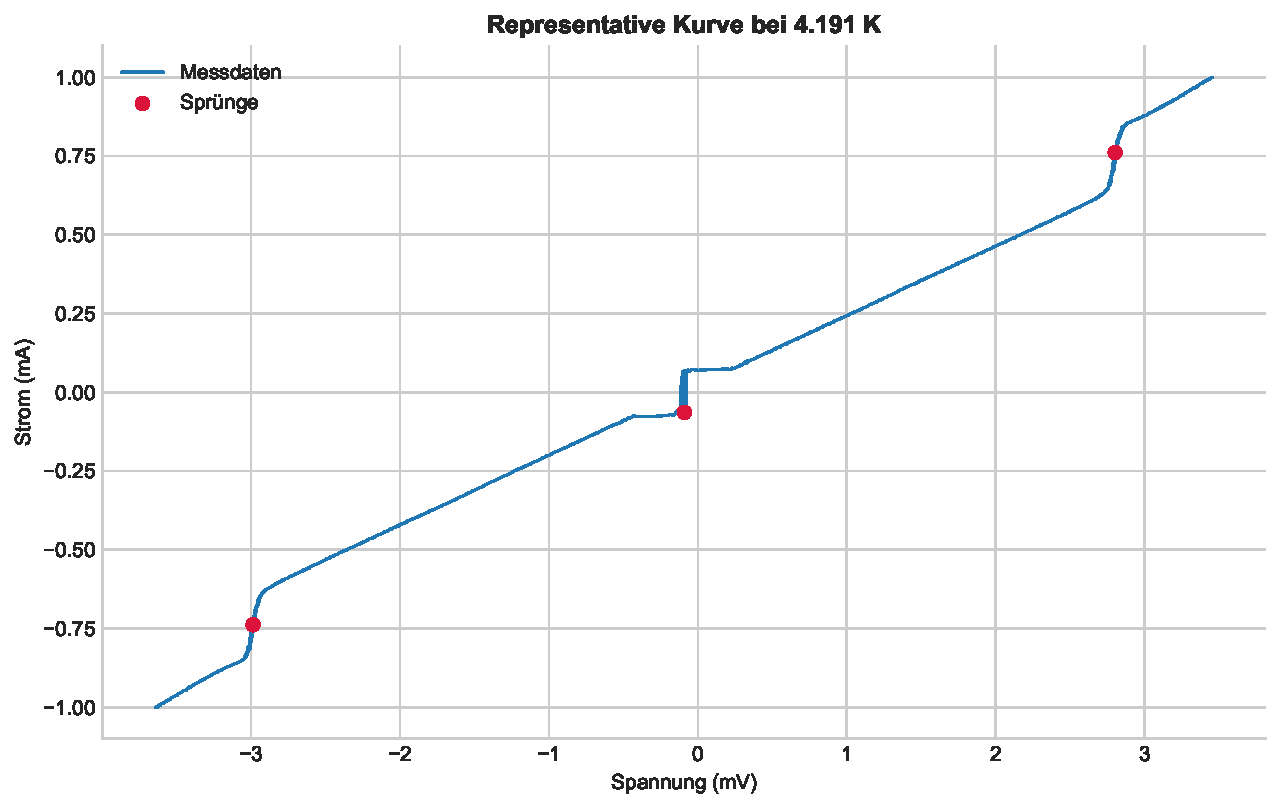
\includegraphics[width=0.8\linewidth]{Leonard/Plots/example_curve.pdf}
        \caption{Es ist die gemessene Strom-Spannungs-Kennlinie bei einer Temperatur von $T = \SI{4.2}{\kelvin}$ zu sehen. Die Sprünge drei Sprünge jeweils sind mit einem roten Punkten markiert.}
        \label{fig:IVT}
    \end{centering}
\end{figure}
Ähnlich wie in \ref{BFeld} lässt sich mit Hilfe eines Fits der kritische Strom $I_\mathrm{c}$ bestimmen. Dies wird für die bei verschiedenen Temperaturen aufgenommenen Kennlinien gemacht. In Abbildung \ref{fig:IT} sind die Werte des reduzierten kritischen Stroms $I_\mathrm{c}(T)/I_{\mathrm{c}}(0)$ gegen die reduzierte Temperatur $T/T_\mathrm{c}$ aufgetragen. Zusätzlich ist theoretische Kurve nach Gleichung bei der kritischen Temperatur von Nyobium von $T_\mathrm{c} = \SI{9.2}{\kelvin}$ eingezeichnet.
\begin{figure}[H]
    \begin{centering}
        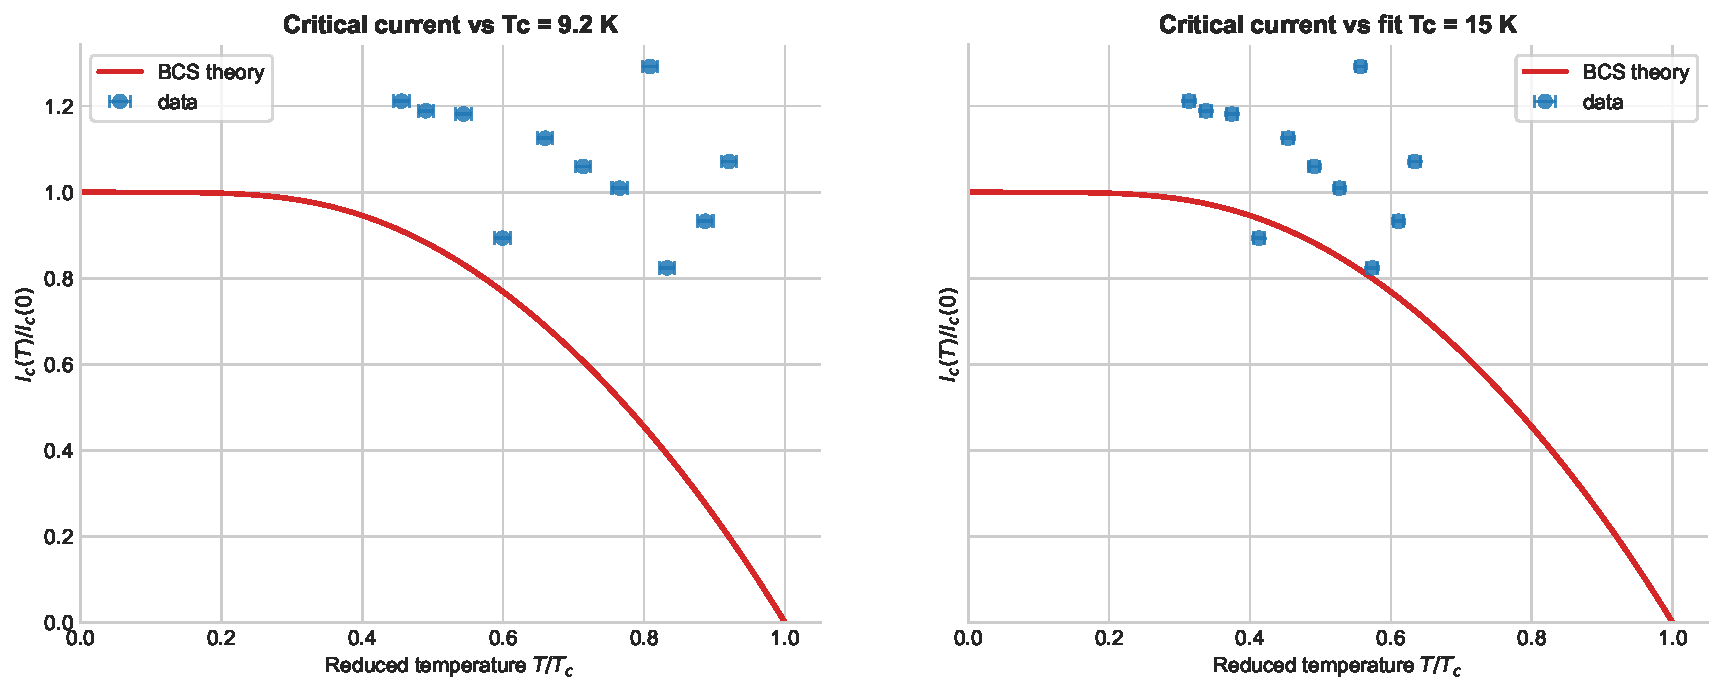
\includegraphics[width=0.8\linewidth]{Leonard/Plots/Ic.pdf}
        \caption{Kritischer Strom $I_\mathrm{c}(T) / I_\mathrm{c}(0)$ gegen reduzierte Temperatur $T / T_\mathrm{c}$. Links für Literaturwerte von $T_\mathrm{c} = \SI{9.2}{\kelvin}$ und rechts für den Fit der kritischen Temperatur $T_\mathrm{c} = \SI{15}{\kelvin}$.}
        \label{fig:IT}
    \end{centering}
\end{figure}

Die Energie-Lücke $\Delta(T)$ kann aus den Sprüngen bei $V = \pm 2\Delta/e$ bestimmt werden. In Abbildung \ref{fig:Delta} ist die Energie-Lücke $\Delta(T) / \Delta(0)$ gegen die reduzierte Temperatur $T / T_\mathrm{c}$ aufgetragen. Zusätzlich ist die theoretische Kurve nach Gleichung \ref{eq:DeltaT} bei der kritischen Temperatur von Nyobium von $T_\mathrm{c} = \SI{9.2}{\kelvin}$ eingezeichnet.
\begin{figure}[H]
    \begin{centering}
        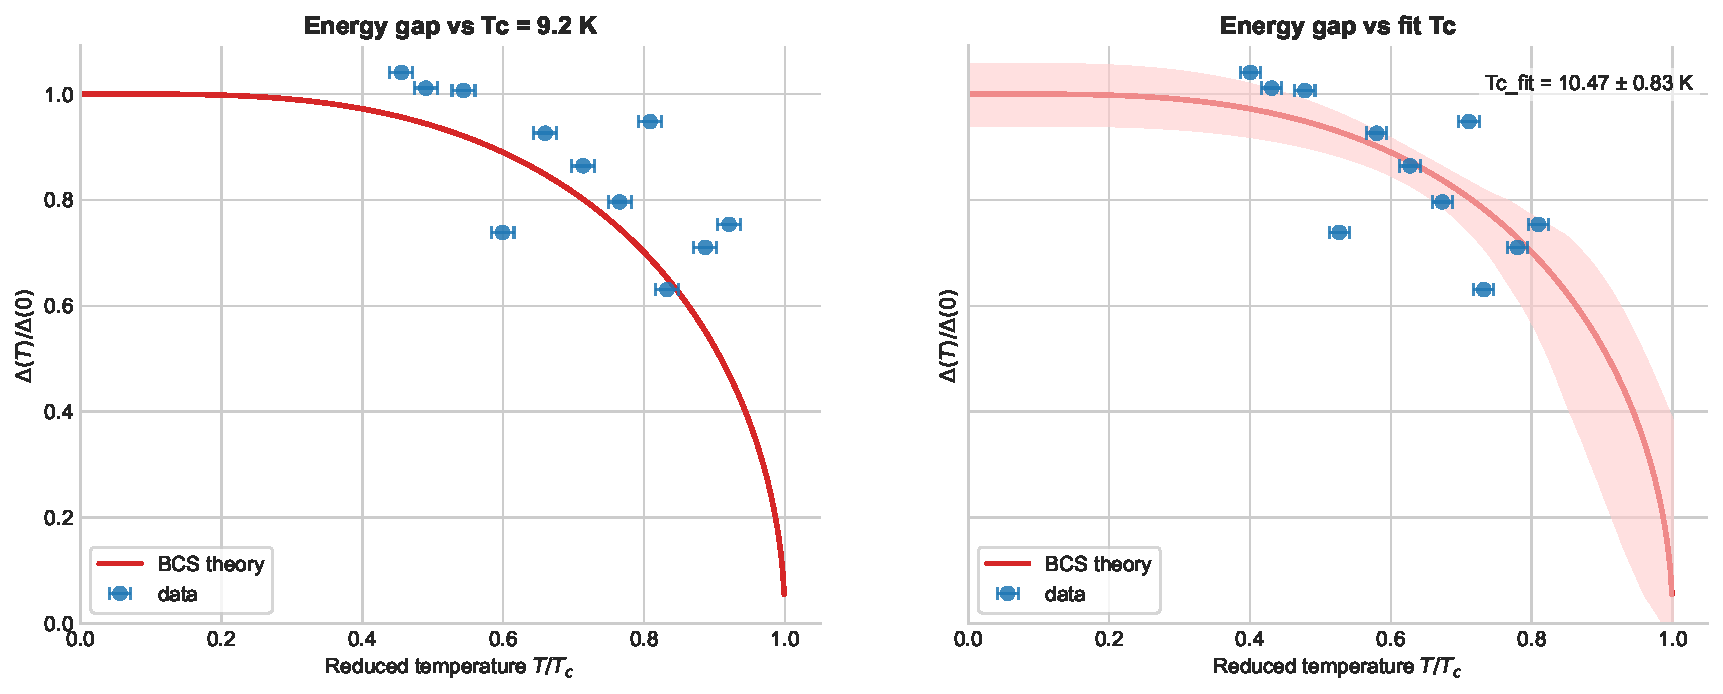
\includegraphics[width=0.8\linewidth]{Leonard/Plots/Delta.pdf}
        \caption{Energie-Lücke $\Delta(T) / \Delta(0)$ gegen reduzierte Temperatur $T / T_\mathrm{c}$. Links für Literaturwerte von $T_\mathrm{c} = \SI{9.2}{\kelvin}$ und rechts für den Fit der kritischen Temperatur $T_\mathrm{c} = \SI{10.5}{\kelvin}$.}
        \label{fig:Delta}
    \end{centering}
\end{figure}
